% !TeX root = ../solution.tex

\hypertarget{he22.19}{%
\chapter{[HE22.19] Ghost in a Shell 3}\label{he22.19}}

\begin{marginfigure}
	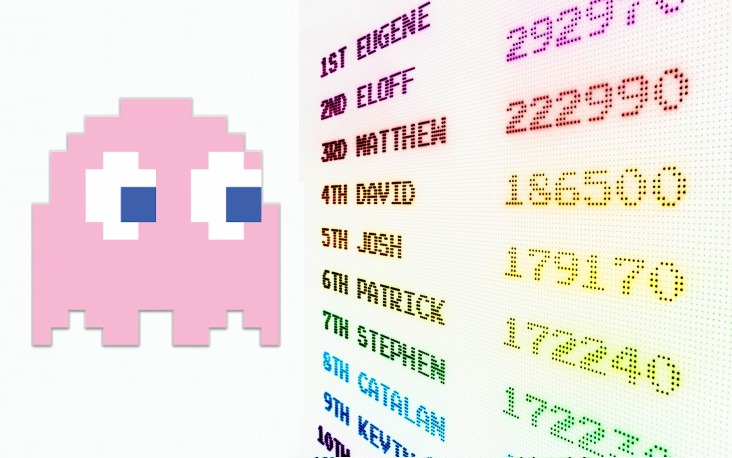
\includegraphics[width=49mm]{level5/challenge19.jpg}
\end{marginfigure}
\subsection{Intro}
\begin{fullwidth}
	{\tiny
\begin{verbatim}
  _, _,_  _,  _, ___   _ _, _    _,    _, _,_ __, _,  _,    ,  ,  ,  
 / _ |_| / \ (_   |    | |\ |   /_\   (_  |_| |_  |   |     |  |  |  
 \ / | | \ / , )  |    | | \|   | |   , ) | | |   | , | ,   |  |  |  
  ~  ~ ~  ~   ~   ~    ~ ~  ~   ~ ~    ~  ~ ~ ~~~ ~~~ ~~~   ~  ~  ~  
______________________________________________________________________  
 ,--.     ,--.     ,--.  
| oo |   | oo |   | oo |   
| ~~ |   | ~~ |   | ~~ |   o  o  o  o  o  o  o  o  o  o  o  o  o  o  o  
|/\/\|   |/\/\|   |/\/\|     
______________________________________________________________________  
  
\end{verbatim}
}
\end{fullwidth}

\noindent Connect to the server, snoop around, and find the flag!
\begin{itemize}
\item \verb+ssh 46.101.107.117 -p 2203 -l pinky+
\item password is: \verb+!speedy!+
\end{itemize}

Note: The service is restarted every hour at x:00.

\section{Solution}\label{hv22.19solution}
In the home directory are two files:

\begin{fullwidth}
	{\tiny
\begin{verbatim}
b6c464bd8644:~$ ls -l
total 8
-rw-r--r--    1 root     root            64 May 21 10:24 flag.enc
-r--------    1 root     root            32 Mar 13 18:22 flag.txt
b6c464bd8644:~$ 
\end{verbatim}
}
\end{fullwidth}

Some snooping around finds a file \verb+/opt/bannerkoder/cipher.sh+ with these contents:

\begin{fullwidth}
	{\tiny
\begin{verbatim}
#!/bin/bash
date +%s | md5sum | base64 | head -c 32 > /tmp/7367111C2875730D00686C13B98E7F36
openssl enc -aes-256-cbc -e -in /home/pinky/flag.txt -out /home/pinky/flag.enc -kfile /tmp/7367111C2875730D00686C13B98E7F36
\end{verbatim}
}
\end{fullwidth}

So we can decode the file with the command
\begin{fullwidth}
	{\tiny
\begin{verbatim}
openssl enc -aes-256-cbc -d -in  /home/pinky/flag.enc -kfile /tmp/7367111C2875730D00686C13B98E7F36
\end{verbatim}
}
\end{fullwidth}
which prints the flag \verb+he2022{0p3n-35-35-37-f0r-pr0fit}+.
	









